\let\negmedspace\undefined
\let\negthickspace\undefined
\documentclass[journal,12pt,onecolumn]{IEEEtran}
\usepackage{cite}
\usepackage{amsmath,amssymb,amsfonts,amsthm}
\usepackage{algorithmic}
\usepackage{graphicx}
\usepackage{textcomp}
\usepackage{xcolor}
\usepackage{txfonts}
\usepackage{listings}
\usepackage{enumitem}
\usepackage{mathtools}
\usepackage{gensymb}
\usepackage{comment}
\usepackage[breaklinks=true]{hyperref}
\usepackage{tkz-euclide} 
\usepackage{listings}
\usepackage{gvv}                                        
\def\inputGnumericTable{}                                 
\usepackage[latin1]{inputenc}                                
\usepackage{color}                                            
\usepackage{array}                                            
\usepackage{longtable}                                       
\usepackage{calc}                                             
\usepackage{multirow}                                         
\usepackage{hhline}                                           
\usepackage{ifthen}                                           
\usepackage{lscape}

\newtheorem{theorem}{Theorem}[section]
\newtheorem{problem}{Problem}
\newtheorem{proposition}{Proposition}[section]
\newtheorem{lemma}{Lemma}[section]
\newtheorem{corollary}[theorem]{Corollary}
\newtheorem{example}{Example}[section]
\newtheorem{definition}[problem]{Definition}
\newcommand{\BEQA}{\begin{eqnarray}}
\newcommand{\EEQA}{\end{eqnarray}}
\newcommand{\define}{\stackrel{\triangle}{=}}
\theoremstyle{remark}
\newtheorem{rem}{Remark}
\begin{document}

\bibliographystyle{IEEEtran}
\vspace{3cm}


\title{Question 41.2023}
\author{EE22BTECH11051}

\maketitle
\vspace{3cm}

\textbf{Question:} \\
Suppose that $X_1$,$X_2$, ...,$X_{10}$ are independen and identically distributed random vectors each having
$N_2(\mu,\Sigma)$ distribution, where $\Sigma$ is non-singular. If
\begin{align}
    \text{U} = \frac{1}{1+(\bar{X} - \mu)^T\Sigma^{-1}(\bar{X} - \mu)} ,
\end{align}
where $\bar X = \frac{1}{10}\Sigma_{i = 1}^{10} X_{i}$ then the value of $\log_e \pr {U \le \frac{1}{2}}$ equals

\begin{enumerate}
    \item -5
    \item -10
    \item -2
    \item -1
\end{enumerate}
\hfill {GATE ST 2023}\\
\textbf{Solution:}\\
\begin{table}[h!]
    \begin{center}
       \begin{tabular}{|l|c|r|}
       \hline
       Parameter & Values & Description\\
       \hline
       $n$ & 10 & Number of random vectors\\
       \hline
       $\mu$ &  & mean\\
       \hline
       $\Sigma$ &  & Covariance\\
       \hline
       \end{tabular}
       \end{center}
   \end{table}
   
We are given a bivariate distribution;
\begin{align}
    X_{i} \sim N_2(\mu,\Sigma)\\
\end{align}
The distribution of $\bar{X}$ can be given as: \\

The mean of $\bar{X}$ will be the average of the means of X1, X2, ..., X10, which is:
\begin{align}
    \mu_{\bar{X}} =\frac{\mu + \mu + \mu + ... + \mu}{10} = \frac{10\mu}{10} = \mu   
\end{align}
And since the distributions $X_1$,$X_2$, ...,$X_{10}$ are independent, the covariance between them is zero. Hence we can find 
the new covariance as:\\
\begin{align}
    \text{Cov}(\bar{X}) = E[(\bar{X}-\mu)(\bar{X}-\mu)^T]\\
     &= E[(\frac{1}{10}\Sigma_{i = 1}^{10} X_{i} - \mu)(\frac{1}{10}\Sigma_{j = 1}^{10} X_{j} - \mu)^T] \\
     &= E[\frac{1}{100}\Sigma_{i = 1}^{10}\Sigma_{j = 1}^{10}(X_{i} - \mu)(X_{j} - \mu)^T]\\
     &= \frac{1}{100}\Sigma_{i = 1}^{10}\Sigma_{j = 1}^{10}E[(X_{i} - \mu)(X_{j} - \mu)^T]
\end{align}
Since $X_1$,$X_2$, ...,$X_{10}$ are independen and identically distributed random vectors, we get the covariance term $E[(X_{i} - \mu)(X_{j} - \mu)^T]$
to be $\Sigma$
hence;
\begin{align}
    \text{Cov}(\bar{X}) = \frac{1}{100}\times10\times\Sigma\\
    \bar{X} \sim N_2\brak{\mu,\frac{\Sigma}{n}}
\end{align}
let's define $Z$ as follows:
\begin{align}
     Z = \sqrt{10}\Sigma^{-1/2}(\bar{X} - \mu)
\end{align}

Now, express $U$ in terms of $Z$:
\begin{align}
    U = \frac{1}{1 + (\bar{X} - \mu)^T \Sigma^{-1} (\bar{X} - \mu)}
    = \frac{1}{1 + Z^T Z}
\end{align}

Now, the distribution of $Z$ is $N_2(0, I)$ (a multivariate normal distribution with mean $0$ and covariance matrix $I$). Therefore, the expression for $U$ becomes:
\begin{align}
    U = \frac{1}{1 + \|Z\|^2}
\end{align}

where $\|Z\|^2$ is the squared Euclidean norm of $Z$.\\

Now, the probability $\Pr(U \leq \frac{1}{2})$ is equivalent to 
\begin{align}
    \Pr\left(\frac{1}{1 + \|Z\|^2} \leq \frac{1}{2}\right)
    = \Pr(\|Z\|^2 \geq 1)
\end{align}


The term $\|Z\|^2$ follows a $\chi^{2}_{2}$ distribution, and we are looking for $\log_e \Pr(\|Z\|^2 \geq 1)$.\\

Since $k=2$ for Y, we get;
\begin{align}
    &= \int_{10}^{\infty} \frac{1}{2}e^{-\frac{y}{2}} \,dy\\
    &= e^{-5}   
\end{align}   

Hence;
\begin{align}
    \log_e \pr{U \le \frac{1}{2}} = -5
\end{align}

\textbf{Simulation Steps:}
\begin{enumerate}
    \item Set the number of simulations
    \item Run a loop for number of simulations specified
    \item Generate random vectors from a bivariate normal distribution
    \item Calculate the sample mean and set the covariance matrix
    \item Using the given formula, calculate U for each simulation
    \item Calculate the simulated probability adn take the natural log of that value
\end{enumerate}

\begin{figure}[!ht]
    \centering
    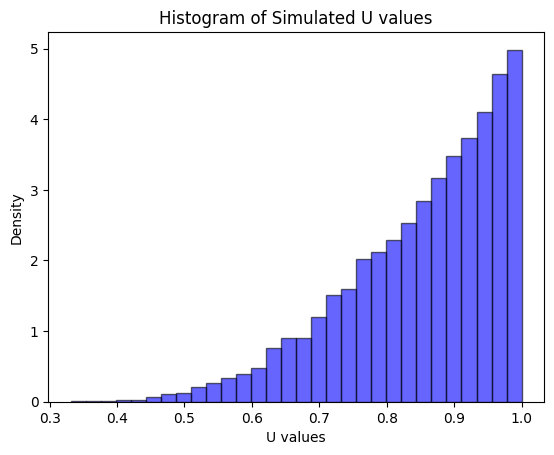
\includegraphics[width=\columnwidth]{./figs/sim.png}
    \caption{Plot of $p_X(n)$.Simulations are close to the analysis. }
    \end{figure}



\end{document}